The Liaison System is created to assure that the correct data collected from a microcontrollers is received correctly by the end user.
To achieve this, the system uses four equal but distinct microcontrollers, an internal voting system to assure that if any of the microcontrollers
disagree, it is marked as malfunctioning and is no longer allowed to send output. The output from the Liaison is extended with a system status
code that tells the end user if any of the microcontrollers are damaged, and the signal is then enhanced with an error correcting code such that
we can be more certain that the signal is not distorted on its way to the reciever.

\begin{figure}[h]
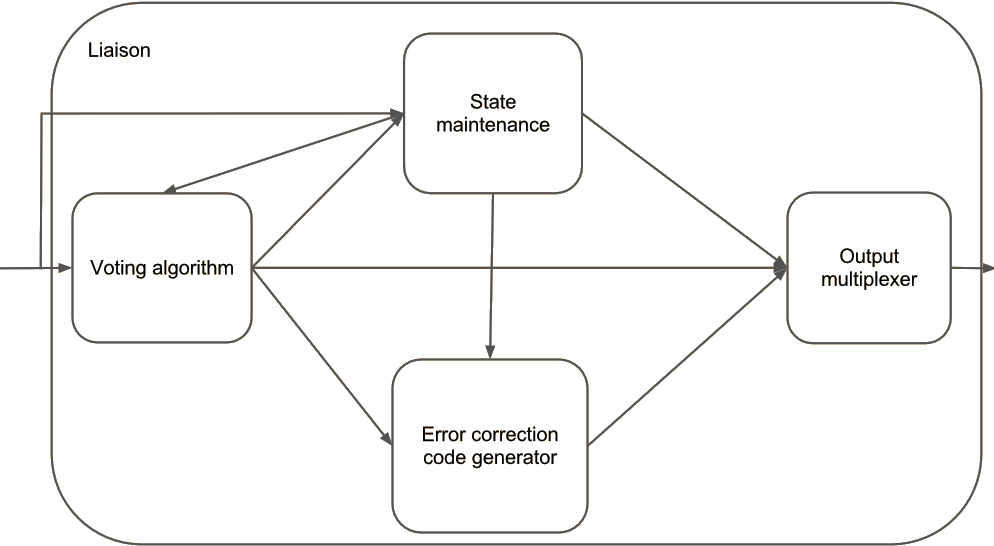
\includegraphics[width=15cm]{design/fig_overview}
\caption{Modules overview}
\label{fig:overview}
\end{figure}

As we can see from \autoref{fig:overview}, the internals of the Liaison can be modeled as four different pieces of hardware, each providing a
nessesary service to the system.

\subsection{Voting algorithm}
The system needs to distinguish between the working and the malfunctioning microcontrollers. To do this, the voting module knows what microcontrollers
that has shown sign of failure from earlier voting, and it needs to vote for the majority result of working microcontrollers. This modules
receives input directly from the microcontrollers, and it gets the current system state from the State Maintainance module.

\subsection{State maintainance}
The State Maintainance module is responsible for all internal states of the system. The system keeps track of what microcontrollers that can
no longer be trusted. This works by tagging those microcontrollers were the signal differs from the voted signal from the Voter module. When
a microcontroller has been tagged, the tag is not cleared until the entire system is reset.

This modules also outputs a system status vector as part of the Liaison output. This vector has one of four states as shown in \autoref{tab:systemstatus}.
The output status is a direct mapping from the internal tag-vector, and works simply as a lookup table.

At last, the State Maintainance module is also responsible for counting what output is sent at each clock tick. Since we are outputing a serial data stream
where different sections of the stream have different sources (data, status, ECC), we need to keep track of the position of the current data bit.

\subsection{Error Correcting Code Generator}
To provide reliable output for long distance transmission of data, the Liaison System adds an error correcting code to its data packets. The Error
Correcting Code Generator generates (16,11)-Hamming code on the fly and attaches the code at the end of the output stream. This module uses information
from the Voter to get the first 8 data bits and information from the State Maintainance to get the status word. It also uses information on current 
data bit position from the State Maintainance module, since Hamming Code is generated using parity of bits at specific positions\cite{ecc}.

When (16,11)-Hamming code is used, we are able to correct a single error in the packet, but we are also able to detect up to two errors in the same packet.
The first 4 bits in the Hamming code is used for error correction of a single bit, and the additional bit adds the ability to detect another error.

\subsection{Output mulitplexer}
Since the Liaison System needs to send output from each of the three other modules at specific clock cycles when specific events has occured, we need
a logic piece of hardware that can multiplex all modules and allways output the correct signal. The Output Multiplexer uses the position of current data bit
from the State Maintainance module to select what module to send data from.
